\documentclass[preview]{standalone}

\usepackage[usenames,dvipsnames]{xcolor}
\usepackage{tikz,ifthen,fullpage}
\usetikzlibrary{intersections}
\usetikzlibrary{math}

\begin{document}
\thispagestyle{empty}
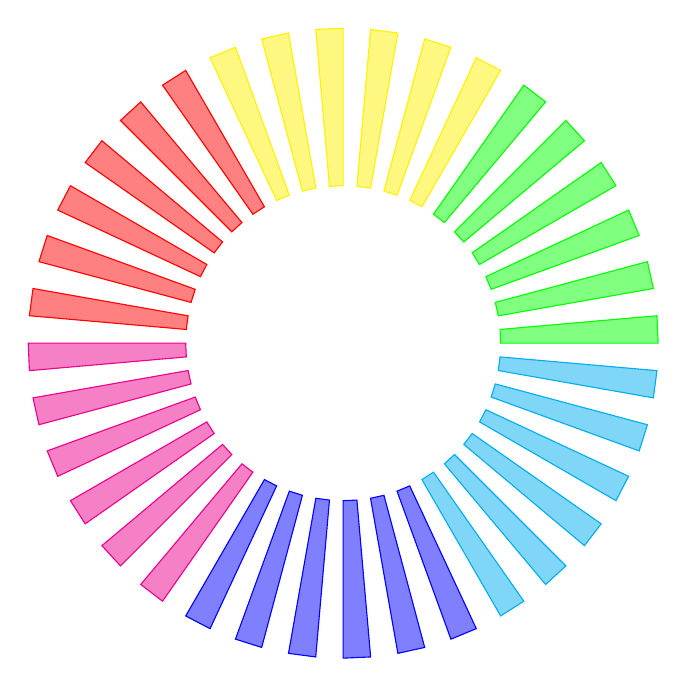
\begin{tikzpicture}
\tikzmath{
  int \x;
  for \k in {0,10,...,350}{
    if \k>290 then { let \c = cyan; } else {
      if \k>230 then { let \c = blue; } else {
        if \k>170 then { let \c = magenta; } else {
          if \k>110 then { let \c = red; } else {
            if \k > 50 then { let \c = yellow; } else {
              let \c = green; }; }; }; }; };
{
\path [fill=\c!50, draw=\c] (\k:2cm) -- (\k:4cm) --
        (\k+5:4cm) -- (\k+5:2cm) -- cycle;
    };
}; }
\end{tikzpicture}
\end{document}
